\documentclass[letterpaper]{article}
% Required Packages
\usepackage{acl-hlt2011}
\usepackage{times}
\usepackage{helvet}
\usepackage{courier}

% The packages I added.
\usepackage{graphicx}
\usepackage{url}
\usepackage{multicol}
\usepackage{tabularx}
\usepackage{varwidth}
\usepackage{threeparttable}
\usepackage{listings}
\usepackage{algorithm}

\newcommand{\war}[1]{{\sf\small #1}}
\frenchspacing

%%%%%%%%%%
% PDFMARK for TeX and GhostScript
% Uncomment and complete the following for
% metadata if your paper is typeset using TeX and
% GhostScript (e.g if you use .ps or .eps files in your paper):
% \special{! /pdfmark where
% {pop} {userdict /pdfmark /cleartomark load put} ifelse
% [ /Author (John Doe, Jane Doe)
% /Title (Input Your Paper Title Here)
% /Subject (Input the Proceedings Title Here)
% /Keywords (Input your paper��s keywords here)
% /DOCINFO pdfmark
%}
%%%%%%%%%%
% PDFINFO for PDFTEX
% Uncomment and complete the following for metadata if
% your paper is typeset using PDFTEX
%\pdfinfo{
%/Title WikiTopics: What is popular on Wikipedia and why
%/Author Byung Gyu Ahn, Chris Callison-Burch, Benjamin Van Durme
%/Subject AAAI-11
%/Keywords Topic detection and tracking, Wikipedia
%}
%%%%%%%%%%
% Section Numbers
% Uncomment if you want to use section numbers
% and change the 0 to a 1 or 2
% \setcounter{secnumdepth}{0}
%%%%%%%%%%
% Title, Author, and Address Information
\title{WikiTopics: What is popular on Wikipedia and why}
%\author{Byung Gyu Ahn
%\and Chris Callison-Burch
%\and Benjamin Van Durme\\
%Center for Language and Speech Processing\\
%Johns Hopkins University\\
%Baltimore, Maryland\\
%{\tt \{bahn, ccb, vandurme\}@cs.jhu.edu}}
%%%%%%%%%%
% Body of Paper Begins
\begin{document}
\maketitle

\begin{abstract}
We establish a novel task in the spirit of news summarization and topic detection and tracking (TDT): daily determination of the topics newly popular with Wikipedia readers.  Central to this effort is a new public dataset consisting of the hourly page view statistics of all Wikipedia articles over the last three years.  We give baseline results for the tasks of: discovering individual pages of interest, clustering these pages into coherent topics, and extracting the most relevant summarizing sentence for the reader.  When compared to human judgements, our system shows the viability of this task, and opens the door to a range of exciting future work.

\end{abstract}

\section{Introduction}
In this paper we analyze a novel dataset: we have collected the hourly page view statistics\footnote{http://dammit.lt/wikistats} for every Wikipedia page in every language for the last three years. We show how these page view statistics, along with other features like article text and inter-page hyperlinks, can be used to identify and explain popular trends, including popular films and music, sports championships, elections, natural disasters, etc.

Our approach is to select a set of articles whose daily pageviews for the last fifteen days increase above those of the previous fifteen days. Rather than simply selecting the most popular articles for a given day, this selects articles whose popularity is rapidly increasing. These popularity spikes tend to be due to significant current events in the real world. We examine 100 such articles for each of 5 randomly selected days in 2009 and attempt to group the articles into clusters such that the clusters coherently correspond to current events and extract a summarizing sentence that best explains the relevant event. Quantitative and qualitative analyses are provided along with the evaluation dataset.

We compare our automatically collected articles to those in the current events portal of Wikipedia where Wikipedia editors manually chronicle current events every day, which comprise armed conflicts, international relations, law and crime, natural disasters, social, political, sports events, etc. Each event is summarized into a simple phrase or sentence along with links to related articles. We view our work as an automatic mechanism that could potentially supplant this hand-curated method of selecting current events by editors.

\begin{figure}
\centering
\begin{tabular}{|c|}
\hline
\war{Barack Obama} \\
\war{Joe Biden} \\
\war{White House} \\
\war{Inauguration} \\
\dots \\
\war{US Airways Flight 1549} \\
\war{Chesley Sullenberger} \\
\war{Hudson River} \\
\dots \\
\war{Super Bowl} \\
\war{Arizona Cardinals} \\
\hline
\end{tabular}
\caption{Automatically selected articles for Jan 27, 2009.}
\label{fig:topics-jan-27}
\end{figure}

Figure~\ref{fig:topics-jan-27} shows examples of automatically selected articles for January 27, 2009. We would group the articles into 3 clusters, \{\war{Barack Obama}, \war{Joe Biden}, \war{White House}, \war{Inauguration}\} which corresponds to the inauguration of Barack Obama, \{\war{US Airways Flight 1549}, \war{Chesley Sullenburger}, \war{Hudson River}\} which corresponds to the successful ditching of an airplane into the Hudson river without loss of life, and \{\war{Superbowl}, \war{Arizona Cardinals}\} which corresponds to the then upcoming Superbowl XLIII.

We further try to explain the clusters by selecting sentences from the articles. For the first cluster, a good selection would be ``the inauguration of Barack Obama as the 44th president \ldots took place on January 20, 2009''. For the second cluster, ``Chesley Burnett `Sully' Sullenberger III (born January 23, 1951)  is an American commercial airline pilot, \ldots, who successfully carried out the emergency water landing of US Airways Flight 1549 on the Hudson River, offshore from Manhattan, New York City, on January 15, 2009, \ldots'' would be a nice summary, which also provides links to the other articles in the same cluster. For the third cluster, ``Superbowl XLIII will feature the American Football Conference champion Pittsburgh Steelers (14-4) and the National Football Conference champion Arizona Cardinals (12-7) .'' would be a good choice which delineates the association with \war{Arizona Cardinals}.

Different clustering methods and sentence selection features are evaluated and results are compared. Topic models, such as K-means \cite{manning08ir} clustering in vector space model and latent Dirichlet allocation \cite{blei03lda}, are compared to clustering using Wikipedia's link structure. To select sentences we make use of NLP technologies such as coreference resolution, named entity and date taggers. Note that the latest revision of each article as of the day on which the article is selected is used in clustering and textualization to simulate the situation in which article selection, clustering, and textualization are performed once every day.

Figure~\ref{fig:process} illustrates the pipeline of our WikiTopics system: article selection, clustering, and textualization.

\begin{figure*}
\centering
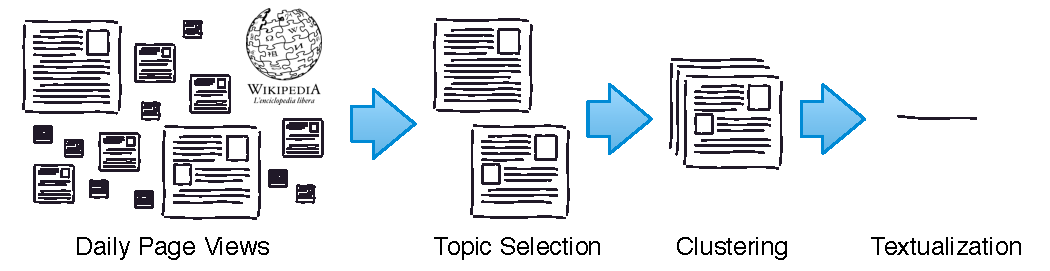
\includegraphics[width=0.8\textwidth]{figures/WikiTopicsPipeline.pdf}
\caption{Process diagram:
(a) Topic selection: select interesting articles based on increase in pageviews.
(b) Clustering: cluster the articles according to relevant events using topic models or Wikipedia's hyperlink structure.
(c) Textualization: select the sentence that best summarizes the relevant event.}
\label{fig:process}
\end{figure*}

\section{Article selection}

We would like to identify an uptrend in popularity of articles. In an online encyclopedia such as Wikipedia, the pageviews for an article reflect its popularity. Following the Trending Topics software\footnote{http://www.trendingtopics.org}, WikiTopics's articles selection algorithm determines each articles' monthly trend value as increase in pageviews within last 30 days. The monthly trend value $t^k$ of an article $k$ is defined as below:
$$ t^k = \sum_{i=1}^{15} d_i^k - \sum_{i=16}^{30} d_i^k $$
where
$$ d_i^k = \mbox{daily pageviews $i-1$ days ago of an article $k$} $$
We selected 100 articles of the highest trend value for each day in 2009. We call the articles WikiTopics articles. We leave as future work other possibilities to determine the trend value and choose articles\footnote{For example, one might leverage additional signals of real world events, such as Twitter feeds, etc.}, and only briefly discuss some alternatives in this section.

%\begin{algorithm}[t]
%\lstset{language=c++,
%basicstyle=\scriptsize,
%breaklines=true,
%identifierstyle=\ttfamily}
%\begin{lstlisting}
%int calc_trend(int date, int[] pageviews)
%{
%	// pageview[date] is today's pageview counts,
%	// pageview[date-i] is the pageviews i days ago. 
%	int trend_2 = 0;
%	for (int i=0; i<15; i++) {
%		trend_2 += pageviews[date - i];
%	}
%	int trend_1 = 0;
%	for (int i=15; i<30; i++) {
%		trend_1 += pageviews[date - i];
%	}
%	int monthly trend = trend_2 - trend_1;
%	return monthly trend;
%}
%\end{lstlisting}
%\caption{Algorithm to determine trend values.}
%\label{fig:calc-trend}
%\end{algorithm}

\begin{figure}
\centering
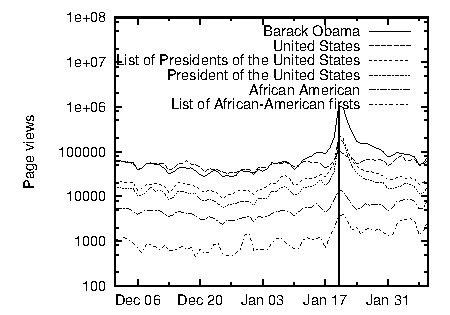
\includegraphics[width=0.5\textwidth]{figures/obama.pdf}
\caption{Pageviews for all the hand-curated articles related to the inauguration of Barack Obama. Pageviews spike on the same day as the event took place--January 20, 2009.}
\label{fig:obama-sparkline}
\end{figure}

%%% hand-curated current events
Wikipedia has a portal page called ``current events'', in which significant current events are listed manually by Wikipedia editors. Figure~\ref{fig:obama-sparkline} illustrates spikes in pageviews of the hand-curated articles related to the inauguration of Barack Obama\footnote{We set up a website where you can see the sparkline graphs of pageviews for every hand-curated event in 2009: http://ANONYMIZED}, which shows clear correlation between the spikes and the day on which the relevant event took place.  It is natural to contrast WikiTopics articles to this set of hand-curated articles. We evaluated WikiTopics articles against hand-curated articles as gold standard and had negative results with precision of 0.13 and recall of 0.28.

%% why they are not good
There are a few reasons for this.  First, there are much fewer hand-curated articles than WikiTopics articles: 17,253 hand-selected articles vs 36,400\footnote{One day is missing from our 2009 pageviews statistics.} WikiTopics articles; so precision cannot be higher than 47\%.  Second, many of the hand-selected articles turned out to have very low pageviews: 6,294 articles (36.5\%) have maximum daily pageviews less than 1,000 whereas WikiTopics articles have increase in pageviews of at least 10,000. It is extremely hard to predict the hand-curated articles based on pageviews. Figure~\ref{fig:logratio} further illustrates hand-curated articles' lack of increase in pageviews as opposed to WikiTopics articles. On the contrary, nearly half of the hand-curated articles have decrease in pageviews. For them, spikes in pageviews are rather an exception than a commonality.  It is concluded that it is futile to predict hand-curated articles based on pageviews.  The hand-curated articles suffer from low popularity and do not spike in pageviews often.
\begin{figure}
\centering
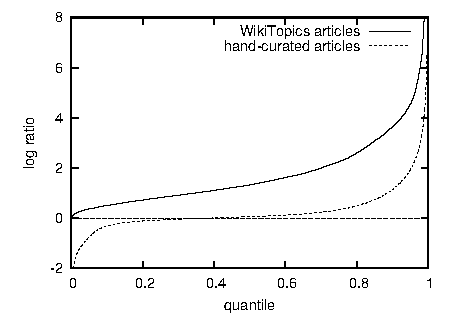
\includegraphics[width=0.5\textwidth]{figures/logratio.pdf}
\caption{Log ratio of the increase in pageviews: $\log \sum {i=1}^{15} d i^k / \sum {i=16}^{30}$. Zero means no change in pageviews. WikiTopics articles show pageviews increase in a few orders of magnitude as opposed to hand-curated articles.}
\label{fig:logratio}
\end{figure}

%% alternatives
There are various viable alternatives to the monthly trend value. As one of them, we did some preliminary experiments with the daily trend value, which is defined by $ d_1^k - d_2^k $, i.e. the difference of the pageviews between the day and the previous day: we found that articles selected using the daily trend value have little overlap--less than half the articles overlapped with the monthly trend value.  Future work will consider the addition of sources other than pageviews, such as edit histories and Wikipedia category information, along with more intelligent technique to combine these different sources.

%% brief summary of the section
We have introduced the problem and a baseline solution. From now on, we focus on the selected WikiTopics articles.  Figure~\ref{fig:comparison-articles} contrasts the WikiTopics articles and the hand-curated articles. The WikiTopics articles shown here do not appear in the hand-curated articles within fifteen days before or after, and vice versa.  WikiTopics selected articles about people who played a minor role in the relevant event, recently released films, their protagonists, popular TV series, etc.  Wikipedia editors selected articles about actions, things, geopolitical or organizational names in the relevant event and their event description mentions all of them.  We go on further to identify and describe relevant events from WikiTopics articles.

\begin{figure}
\centering
\begin{tabular}{|c|}
\hline
WikiTopics articles \\
\hline
\war{Joe Biden} \\
\war{Notorious (2009 film)} \\
\war{The Notorious B.I.G.} \\
\war{Lost (TV series)} \\
\ldots \\
\hline
hand-curated articles \\
\hline
\war{Fraud} \\
\war{Florida} \\
\war{Hedge fund} \\
\war{Arthur Nadel} \\
\war{Federal Bureau of Investigation} \\
\hline
\end{tabular}
\caption{Illustrative articles for January 27, 2009. WikiTopics articles here do not appear in hand-curated articles within fifteen days before or after, and vice versa. The hand-curated articles shown here are all linked from a single event ``Florida hedge fund manager Arthur Nadel is arrested by the United States Federal Bureau of Investigation and charged with fraud.''}
\label{fig:comparison-articles}
\end{figure}

\section{Clustering}

Clustering plays a central role to identify current events; a group of coherently related articles corresponds to a current event. Clusters, in general, may have hierarchies and an element may be a member of multiple clusters. Whereas Wikipedia's current events are hierarchically compiled into different levels of events, we focus on flat clustering, leaving hierarchical clustering as future work, but allow multiple memberships. In addition to clustering using Wikipedia's inter-page hyperlink structure, we experimented with two families of clustering algorithms pertaining to topic models: K-means clustering in vector space model and latent Dirichlet allocation (LDA) probabilistic topic model. We used the Mallet software \cite{McCallumMALLET} to run the topic models. The latest revision of each article as of the day on which WikiTopics selected the article was retrieved, with unnecessary HTML tags and Wiki templates stripped with mwlib\footnote{http://code.pediapress.com/wiki/wiki/mwlib} and sentences split with NLTK \cite{Loper02NLTK}. Normalization, tokenization, and stop words removal were performed. The unigram (bag-of-words) model was used and the number of clusters/topics $k$ was set to $50$, which is half the number of articles. For K-means, the common settings were used: tf and tf-idf weighting and cosine similarity \cite{Allan:00}. For LDA, we chose the most probable topic for each article as the cluster ID.
%%% clustering with link structure
Two different clustering schemes make use of the inter-page hyperlink structure: ConnComp and OneHop.  In these schemes, the link structure is treated as a graph, in which each page corresponds to a vertice and each link to an undirected edge. ConnComp groups a set of articlces in each connected component together.  OneHop chooses an article and groups a set of articles within one hop away following links, where the number of resulting clusters depends on the order in which you choose an article.  To find the minimum or maximum number of such clusters would be computationally expensive.  Instead of attempting to find the optimal number of clusters, we take a greedy approach and iteratively create clusters that maximize the central node connectivity, stopping when all nodes are in at least one cluster.\footnote{This allows for singleton clusters.}

%%% evaluation dataset and the metric
Three annotators manually clustered WikiTopics articles for five randomly selected days.  The three manual clusters were evaluated against each other to measure inter-annotator agreement, using the multiplicity B$^3$ metric \cite{amigo09}.  Table~\ref{tab:clustering-results} shows the results.
\begin{table}
% table from /Users/bahn/Dropbox/Documents/Research/Wikitopics/Clustering\ Accuracy.xlsx
% CCB is Manual-1, Ben Manual-2, and Bahn Manual-3.
\centering
\begin{tabular}{|ccc|}
\hline
Test set & \# Clusters & B$^3$ F-score \\
\hline
\hline
Human-1 & 48.6 &         0.704  $\pm$        {\small 0.083} \\
Human-2 & 50.0 &         0.710  $\pm$        {\small 0.108} \\
Human-3 & 53.8 & \textbf{0.741} $\pm$ \textbf{\small 0.103} \\
\hline
ConnComp       & 31.8 &         0.424  $\pm$        {\small 0.183} \\
OneHop         & 45.2 &         0.580  $\pm$        {\small 0.172} \\
K-means tf     & 50   &         0.521  $\pm$        {\small 0.042} \\
K-means tf-idf & 50   & \textbf{0.584} $\pm$ \textbf{\small 0.089} \\
LDA            & 44.8 &         0.426  $\pm$        {\small 0.080} \\
\hline
\end{tabular}
\caption{Clustering evaluation: F-scores are averaged across gold standard datasets. ConnComp and OneHop are using the link structure. K-means clustering with tf-idf performs best. Manual clusters were evaluated against those of the other two annotators to determine inter-annotator agreement.}
\label{tab:clustering-results}
\end{table}
The B$^3$ metric is one of the extrinsic clustering evaluation metrics, which need a gold standard set of \emph{categories} to evaluate against. The multiplicity B$^3$ works nicely for overlapping clusters: each item $e$ has potentially multiple gold standard categories, and also potentially multiple clusters.  Let $C(e)$ be the set of the clusters that $e$ belongs to, and $L(e)$ be the set of $e$'s categories.  The multiplicity B$^3$ scores for a pair of $e$ and $e'$ are evaluated as follows:
$$ \mbox{Prec}(e,e') = { \min \left( |C(e) \cap C(e')| , |L(e) \cap L(e')| \right) \over |C(e) \cap C(e')| } $$
$$ \mbox{Recall}(e,e') = { \min \left( |C(e) \cap C(e')| , |L(e) \cap L(e')| \right) \over |L(e) \cap L(e')| } $$
The overall B$^3$ scores are evaluated as follows:
$$ \mbox{Prec} = \mbox{Average} _{e \neq e'} \mbox{Prec}(e,e') $$
$$ \mbox{Recall} = \mbox{Average} _{e \neq e'} \mbox{Recall}(e,e') $$
The inter-annotator agreement in the B$^3$ scores are in the range of 67\%--74\%.  K-means clustering performs best, achieving 79\% precision compared to manual clustering. OneHop clustering using the link structure achieved comparable performance. LDA performed significantly worse, comparable to ConnComp clustering.

\begin{figure}
\begin{tabular}{cc}
\begin{tabular}{|c|}
\hline
\textbf{Airbus A320 family} \\
Air Force One \\
Chesley Sullenberger \\
US Airways Flight 1549 \\
\hline
\end{tabular}
&
\begin{tabular}{|c|}
\hline
\textbf{Super Bowl XLIII} \\
Arizona Cardinals \\
Super Bowl \\
Kurt Warner \\
\hline
\end{tabular}
\end{tabular}

\centering{
\begin{tabular}{|c|}
\hline
\textbf{2009 flu pandemic by country} \\
Severe acute respiratory syndrome \\
2009 flu pandemic in the United States \\
\hline
\end{tabular}
}

\caption{Examples of clusters: K-means clustering on the articles of January 27, 2009 and May 12, 2009. The centroid article for each cluster, defined as the closest article to the center of the cluster in vector space, is in bold.}
\end{figure}

%%% why clustering is hard
Clustering the articles according to the relevance to recent popularity is not trivial even for humans. In WikiTopics articles for February 10, 2009, \war{Journey (band)} and \war{Bruce Springsteen} may seem to be relevant to \war{Grammy Awards}, but in fact they are relevant on this day because of the \war{Super Bowl}.  K-means fails to recognize this and put them into the cluster of \war{Grammy Awards}, while ConnComp merged \war{Grammy Awards} and \war{Super Bowl} into the same cluster.  OneHop kept the two clusters intact and benefited from putting \war{Bruce Springsteen} into both the clusters.  LDA clustering does not have such a benefit; its performance might have suffered from our allowing only a single membership for an article.
%%% clustering using the link structure and octopus articles
Clustering using the link structure performs comparably with other clustering algorithms without using topic models. It is worth noting that there are a few ``octopus'' articles that have links to many articles.  The \war{United States} on January 27, 2009 was disastrous, with its links to 58 articles, causing ConnComp clustering to group 89 articles into a single cluster. OneHop clustering's condition that groups only articles that are one hop away alleviates the issue and it also benefited from putting an article into multiple clusters.

%%% clustering using news articles
To see if external source help better clustering, we explored the use of news articles.  We included the news articles that we crawled from various news websites into the same vector space as the Wikipedia articles, and ran K-means clustering with the same settings as before.  For each day, we experimented with news articles within different numbers of past days.  The results did not show significant improvement over clustering without external news articles.  This needs further investigation.

\section{Textualization}

We would like to generate textual descriptions for the clustered articles to explain why they are popular and what event is relevant.  We started with a two-step approach similar to multi-document extractive summarization approaches.  The first step is sentence selection; we extracts the best sentence that describes the relevant event for each article. The second step is combining the selected sentences of a cluster into a coherent summary.  Here, we focus on the first step of selecting a sentence and evaluate the selected sentences.  The selected sentences for each cluster are then put together without modification, where the quality of generated summary mainly depends on the extracted sentences at the first step.  We consider each article separately, using as features only information such as date expressions and references to the topic of the article. Future work will consider sentence extraction, aware of the related articles in the same cluster, and better summarization techniques, such as sentence fusion or paraphrasing.

We preprocess the Wikipedia articles using the Serif system \cite{BoscheeSerif} for date tagging and coreference resolution.  The identified temporal expressions are in various formats such as exact date (``February 12, 1809''), a season (``spring''), a month (``December 1808''), a date without a specific year (``November 19''), and even relative time (``now'', ``later that year'', ``The following year''). Some examples are shown in Figure~\ref{fig:temporal-expressions}.  The entities mentioned in a given article are compiled into a list and the mentions of each entity, including pronouns, are linked to the entity as a coreference chain.

\begin{figure}
\centering
\begin{multicols}{2}
February 12, 1809 \\
1860 \\
now \\
the 17th century \\
some time \\
December 1808 \\
34 years old \\
spring \\
September \\
Later that year \\
November 19 \\
that same month \\
The following winter \\
The following year \\
April 1865 \\
late 1863
\end{multicols}
\caption{Selected examples of temporal expressions identified by Serif from 247 such date and time expressions extracted from the article \war{Abraham Lincoln}.}
\label{fig:temporal-expressions}
\end{figure}

%%% sentence selection schemes
In our initial scheme, we picked the first sentence of each article because the first sentence is usually an overview of the topic of the article and often relevant to the current event. For example, a person's article often has the first line with one's recent achievement or death. An article about an album or a film often begins with the release date. We call this \textbf{First}.

We also picked the sentence with the most recent date to the day on which the article was selected.  Dates in the near future are considered in the same way as the recent dates.  Dates may appear in various formats, so we make a more specific format take precedence, i.e. ``February 20, 2009'' is selected over vaguer dates such as ``February 2009'' or ``2009''.  We call this scheme \textbf{Recent}.

As the third scheme, we picked the sentence with the most recent date among those with a reference to the article's topic.  The reasoning behind this is if the sentence refers to the topic of the article, it is more likely to be relevant to the current event. We call this scheme \textbf{Self}.

\begin{figure*}
\underline{2009-01-27: \war{Inauguration of Barack Obama}}

\textbf{\small Gold:} {\small The inauguration of Barack Obama as the forty-fourth President of the United States took place on January 20, 2009.} \\
\textbf{\small Second best:} {\small The inauguration, with a record attendance for any event held in Washington, D.C., marked the commencement of the four-year term of Barack Obama as President and Joseph Biden as Vice President.} \\
{\small With his inauguration as President of the United States, Obama became the first African American to hold the office and the first President born in Hawaii.:} \\
{\small Official events were held in Washington, D.C. from January 18 to 21, 2009, including the We Are One: The Obama Inaugural Celebration at the Lincoln Memorial, a day of service on the federal observance of the Martin Luther King, Jr. Day, a "Kids' Inaugural: We Are the Future" concert event at the Verizon Center, the inaugural ceremony at the U.S. Capitol, an inaugural luncheon at National Statuary Hall, a parade along Pennsylvania Avenue, a series of inaugural balls at the Washington Convention Center and other locations, a private White House gala and an inaugural prayer service at the Washington National Cathedral.:} \\
\textbf{\small First:} {\small The inauguration of Barack Obama as the forty-fourth President of the United States took place on January 20, 2009.} \\
\textbf{\small Recent:} {\small On January 22, 2009, a spokesperson for the Joint Committee on Inaugural Ceremonies also announced that holders of blue, purple and silver tickets who were unable to enter the Cap itol grounds to view the inaugural ceremony would receive commemorative items.} \\
\textbf{\small Self:} {\small On January 21, 2009, President Obama, First Lady Michelle Obama, Vice President Biden and Dr. Jill Biden attended an inaugural prayer service at the Washington National Cathedral.} \\

\underline{2009-02-10: \war{February 2009 Great Britain and Ireland snowfall}}

\textbf{\small Gold:} {\small The snowfall across Great Britain and Ireland in February 2009 is a prolonged period of snowfall that began on 1 February 2009.} \\
\textbf{\small Second best:} {\small Many areas experienced their largest snowfall levels in 18 years.} \\
\textbf{\small First:} {\small The snowfall across Great Britain and Ireland in February 2009 is a prolonged period of snowfall that began on 1 February 2009.} \\
\textbf{\small Recent:} {\small BBC regional summary - 4 February 2009} \\
\textbf{\small Self:} {\small The snowfall across Great Britain and Ireland in February 2009 is a prolonged period of snowfall that began on 1 February 2009.} \\

\underline{2009-04-19: \war{Wilkins Sound}}

\textbf{\small Gold:} {\small On 5 April 2009 the thin bridge of ice to the Wilkins Ice Shelf off the coast of Antarctica splintered, and scientists expect it could cause the collapse of the Shelf.} \\
\textbf{\small Second best:} {\small There are reports the shelf has exploded into hundreds of small ice bergs.} \\
{\small On 5 April 2009, the ice bridge connecting part of the ice shelf to Charcot Island collapsed.:} \\
\textbf{\small First:} {\small Wilkins Sound is a seaway in Antarctica that is largely occupied by the Wilkins Ice Shelf.} \\
\textbf{\small Recent:} {\small On 5 April 2009 the thin bridge of ice to the Wilkins Ice Shelf off the coast of Antarctica splintered, and scientists expect it could cause the collapse of the Shelf.} \\
\textbf{\small Self:} {\small On 25 March 2008 a   chunk of the Wilkins ice shelf disintegrated, putting an even larger portion of the glacial ice shelf at risk.} \\

%\underline{2009-05-12: \war{}}

%\framebox{\small Gold} {\small } \\
%\framebox{\small Second best} {\small } \\
%\framebox{\small First} {\small } \\
%\framebox{\small Recent} {\small } \\
%\framebox{\small Self} {\small } \\

\caption{Sentence selection: examples show the strength and weakness of each scheme. \textbf{First} selects the first sentence, and often fails to relate the current event. \textbf{Recent} tend to pinpoint the exact sentence that describes the relevant current event, but fails when there are several sentences with a recent temporal expression. \textbf{Self} helps avoid sentences that does not refer to the topic of the article, but suffers from errors propagated from coreference resolution.}
\label{fig:sentence-selection}
\end{figure*}

%%% pronoun replacement
After selecting a sentence for each cluster, we substitute personal pronouns in the sentence with their proper names.  This step enhances readability of the sentence, which often refers to people by a pronoun such as ``he'', ``his'', ``she'', or ``her'.  The examples of substituted proper names appear in Figure~\ref{fig:pronoun-replacement} in bold face. The Serif system classifies which entity mentions are proper names, but choosing the best reference for a person is not a trivial task: proper names may vary from \textit{John} to \textit{John Kennedy} to \textit{John Fitzgerald ``Jack'' Kennedy}.  We choose the most frequent proper name.

\begin{figure}
\underline{2009-01-27: \war{Barack Obama}}
\vspace{1pt}

\textbf{\small Before:} {\small He was inaugurated as President on January 20, 2009.} \\
\textbf{\small After:} {\small \underline{Obama} was inaugurated as President on January 20, 2009.} \\
\textbf{\small Coref:} {\small \{Barack Obama, Obama, Barack Obama, Sr., Barack Obama as the forty-fourth President, Crain's Chicago Business naming Obama, Michelle Obama\}} \\

\vspace{6pt}
\underline{2009-05-12: \war{Eminem}}
\vspace{1pt}

\textbf{\small Before:} {\small He is planning on releasing his first album since 2004, Relapse, on May 15, 2009.} \\
\textbf{\small After:} {\small \underline{Eminem} is planning on releasing his first album since 2004, Relapse, on May 15, 2009.} \\
\textbf{\small Coref:} {\small \{Eminem\}} \\

\vspace{6pt}
\underline{2009-10-12: \war{Brett Favre}}
\vspace{1pt}

\textbf{\small Before:} {\small He came out of retirement for the second time and signed with the Minnesota Vikings on August 18, 2009.} \\
\textbf{\small After:} {\small \underline{Favre} came out of retirement for the second time and signed with the Minnesota Vikings on August 18, 2009.} \\
\textbf{\small Coref:} {\small \{Brett Favre, Favre, Bonita Favre, Brett's father Irvin Favre, Deanna Favre, Favre (ISBN 978-1590710364) which discusses their personal family and Green Bay Packers family\}} \\

\caption{Selected examples of pronoun replacement:  Personal pronouns are substituted with their proper names, which are in \underline{underlined}. The coreference chain for the entity is also shown; our method correctly avoids names wrongly placed in the chain.  Unlike the first two sentence, the last one is not related to the current event, his victory against Green Bay Packers.}
\label{fig:pronoun-replacement}
\end{figure}

%%% evaluation
For fifty randomly chosen articles over the five selected days, two annotators selected the sentence that best describes why an article gained popularity recently, among 289 sentences per each article on average.  For each article, annotators picked a single best sentence, and possibly multiple second best sentences.  If there is no such single sentence that best describes a relevant event, annotators marked none as the best sentence and listed sentences that partially explain the relevant event as second best sentences.  The evaluation results for all the selection schemes are shown in Table~\ref{tab:sentence-selection-results}. To see inter-annotator agreement, two annotators' selections were evaluated against each other. The other selection schemes are evaluated against both the two annotators' selection and their scores in the table are averaged across the two.  The precision and recall score for best sentences are determined by evaluating a scheme's selection of the best sentences against a gold standard's selection.  To evaluate second-best sentences, precision is measured as the fraction of articles where the test and gold standard selections overlap (share at least one sentence), compared to the total number of articles that have at least one sentence selected according to the test set.  Recall is defined by instead dividing by the number of articles that have at least one sentence selected in the gold standard.

%%% why this is hard
The low inter-annotator agreement for the best sentence selection shows the difficulty of the problem. However, when a sentence selection scheme is evaluated against the two gold standards, its resulting scores are not that different. It seems that there are a set of articles in which it is easy to pick the best sentence that two annotators and automatic selection schemes easily agree on, and the other set of articles in which it is difficult to find such a sentence. In the \textit{easier} articles, the best sentence often includes a recent date expression, which is easily picked up by the Recent scheme. Figure~\ref{fig:sentence-selection} illustrates such cases. In the more difficult articles, there are no such sentences with recent dates. \war{X2 (film)} is such an example; it was released in 2003. The release of the prequel \war{X-Men Origins: Wolverine} in 2009 renewed its popularity and the \war{X2 (film)} article still does not have any recent dates.  There is a more subtle case: the article \war{Farrah Fawcett} includes many sentences with recent dates in a section, which describes the development of a recent event. It is hard to pinpoint the best one among them.

\begin{table}
	\centering
	\begin{tabular}{|c|cc|cc|}
		\hline
		              & \multicolumn{2}{c|}{Best} & \multicolumn{2}{c|}{Second best} \\
		Scheme        & Precision & Recall & Precision & Recall \\
		\hline
		\hline
		Human         & 0.50 & 0.55 & 0.85 & 0.75 \\
		\hline
		First         & 0.14 & 0.20 & 0.33 & 0.40 \\
		Recent        & 0.31 & 0.44 & 0.51 & 0.60 \\
		Self          & 0.31 & 0.36 & 0.49 & 0.48 \\
		Self fallback & \textbf{0.33} & \textbf{0.46} & \textbf{0.52} & \textbf{0.62} \\
		\hline
	\end{tabular}
	\caption{Textualization: evaluation results of sentence selection schemes. Self fallback scheme first tries to select the best sentence as the Self scheme, and if it fails to select one it falls back to the Recent scheme.}
	\label{tab:sentence-selection-results}
\end{table}

%%% error propagation
Sentence selection heavily depends on other NLP components, so errors in them could result in the error in sentence selection. \war{Serena Williams} is an example that the error in sentence splitting propagates to sentence selection. The best sentence manually selected was the first sentence in the article ``Serena Jameka Williams \ldots , as of February 2, 2009, is ranked World No. 1 by the Women's Tennis Association \dots .'' The sentence was disastrously divided into two sentences right after ``No.'' by NLTK during preprocessing.  In other words, the gold standard sentence could not be selected no matter how well selection performs.\footnote{In a small followup experiment, we found splitta \cite{Gillick:09} to give more accurate segmentations, such as not reproducing this particular error.} Another source of error propagation is coreference resolution. The Self scheme limits sentence selection to the sentences with a reference to the articles' topic, and it failed to improve over Recent. In qualitative analysis, $3$ out of $4$ cases that made a worse choice resulted from failing to recognize a reference to the topic of the article. By having it fall back to Recent's selection when it failed to find any best sentence, its performance marginally improved. Improvements of the components would result in better performance of sentence selection.

%%% summary
WikiTopics's current sentence extraction succeeded in generating the best or second best sentence that summarizes the relevant current event for more than half of the articles, in enhanced readability through coreference resolution. For the other difficult cases, it needs to take different strategies rather than looking for the most recent date expressions.  Alternatives may consider references to other related articles.  These are put together to constitute a summary of a current event, where sentence compression, fusion or paraphrasing may help lead to a more succinct summary.

\section{Related work}

WikiTopics's pipeline architecture has a resemblance to that of news summarization systems such as Columbia Newsblaster \cite{McKeown02}. Newsblaster's pipeline is comprised of components for performing web crawls, article text extraction, clustering, classification, summarization, and web page generation. The system processes a constant stream of newswire documents. In contrast, WikiTopics analyzes a static set of articles. Hierarchical clustering like three-level clustering of Newsblaster \cite{Hatzivassiloglou:00} could be applied to WikiTopics to organize current events hierarchically. Summarizing multiple sentences that are extracted from the articles in the same cluster would provide a comprehensive description about the current event. Integer linear programming-based models \cite{Woodsend:10:ACL,Woodsend:10:EMNLP} have proven to be useful to generate summaries while global constraints like length, grammar, and coverage are met.

The problem of Topic Detection and Tracking (TDT) is to identify and follow new events in newswire, and to detect the first story about a new event \cite{Allan:98}. 
\newcite{Allan:00} evaluated a variety of clustering schemes in the vector space model, where the best settings from those experiments were then used in our work.  This was followed recently by \newcite{Petrovic:10}, who took an approximate approach to first story detection, as applied to Twitter in an on-line streaming setting. Such a system might provide additional information to the WikiTopics pipeline by helping to identify and describe current events that have yet to be explicitly described in a Wikipedia article, but where page view logs indicate something new is of interest.

Wikipedia inter-article links have been utilized to construct a topic ontology \cite{Syed:08}, word segmentation corpora \cite{Gabay:08}, or to compute semantic relatedness \cite{Milne:08}. In our work, we found the link structure to be as useful to cluster topically related articles as topic models using article text.

\section{Conclusions}

We have described a pipeline for article selection, clustering, and
textualization in order to identify and describe significant
current events as according to Wikipedia content, and metadata.
Similarly to Wikipedia editors maintaining that site's ``current
events'' pages, we are concerned with neatly collecting articles of
daily relevance, only automatically, and more in line with expressed
user interest (through the use of regularly updated page view logs).
We have suggested that Wikipedia's hand-curated articles cannot be
predicted solely based on pageviews. Clustering
methods based on topic models and inter-article link structure are
shown to be useful to group a set of articles that are coherently
related to a current event. Clustering based on only link structure
achieved comparable performance with clustering based on topic models.
In a third of cases, the sentence that best described a current event
could be extracted from the article text based on temporal expressions
within an article. We employed a coreference resolution system assist
in text generation, for improved readability. As future work, 
sentence compression, fusion, and paraphrasing could be
applied to selected sentences with various strategies to more
succinctly summarize the current events.  Our approach is language
indepedent, and may be applied to multi-lingual current event
detection, exploiting further the online encyclopedia's
cross-language references. Finally, we plan to leverage
social media such as Twitter as an additional signal, especially in
cases where essential descriptive information has yet to be added to a
Wikipedia article of interest.

%\section*{Acknowledgments}

%The first author was supported by Samsung Scholarship.

%We appreciate Wikipedians Domas Mituzas and Fr\'{e}d\'{e}ric Schu\"{u}tz for making the pageviews statistics avaialble and Peter Skomoroch for prividing Trending Topics and answering questions.

\bibliography{ahn}
\bibliographystyle{acl}
\end{document}

